\documentclass{report}

\usepackage{polski} % Pozwala na użycie polskiego. Ustawia między innymi fontenc na T1
\usepackage[utf8]{inputenc} % Informuje o kodowaniu
\usepackage{enumitem}
\usepackage{xcolor}
\usepackage{xcolor}% http://ctan.org/pkg/xcolor
\usepackage{hyperref}% http://ctan.org/pkg/hyperref
\usepackage{indentfirst}

\definecolor{LinkColor}{HTML}{1d5cc1}

\usepackage{tabto}

\usepackage{graphicx} % Pakiet do obrazów
\graphicspath{ {./Obrazy/} } % Folder, z którego będą brane obrazy

% Nie twórz nowych stron
\usepackage{etoolbox}
\makeatletter
% \patchcmd{\chapter}{\if@openright\cleardoublepage\else\clearpage\fi}{}{}{}
\makeatother

\title{Specyfikacja implementacyjna -- Gra w życie}
\author{Krzysztof Dąbrowski i Jakub Bogusz}
\date{\today}

\begin{document}
\maketitle{}

\tableofcontents{}

\chapter{Projekt systemu}

\section{Graficzny interfejs użytkownika}
Graficzny interfejs użytkownika zawarty będzie w pliku \texttt{.fxml}, napisanym ręcznie lub wygenerowanym przez służący do tego program. Następnie zostanie połączony z logiką działania programu przez klasę \texttt{SetupController}. \\
Główne okno programu zawierać będzie 2 zakładki. Każda z nich będzie obsługiwała i przedstawiała działanie jednego automatu komórkowego.
\section{Diagram klas}
\begin{figure}
	\hspace*{-3cm}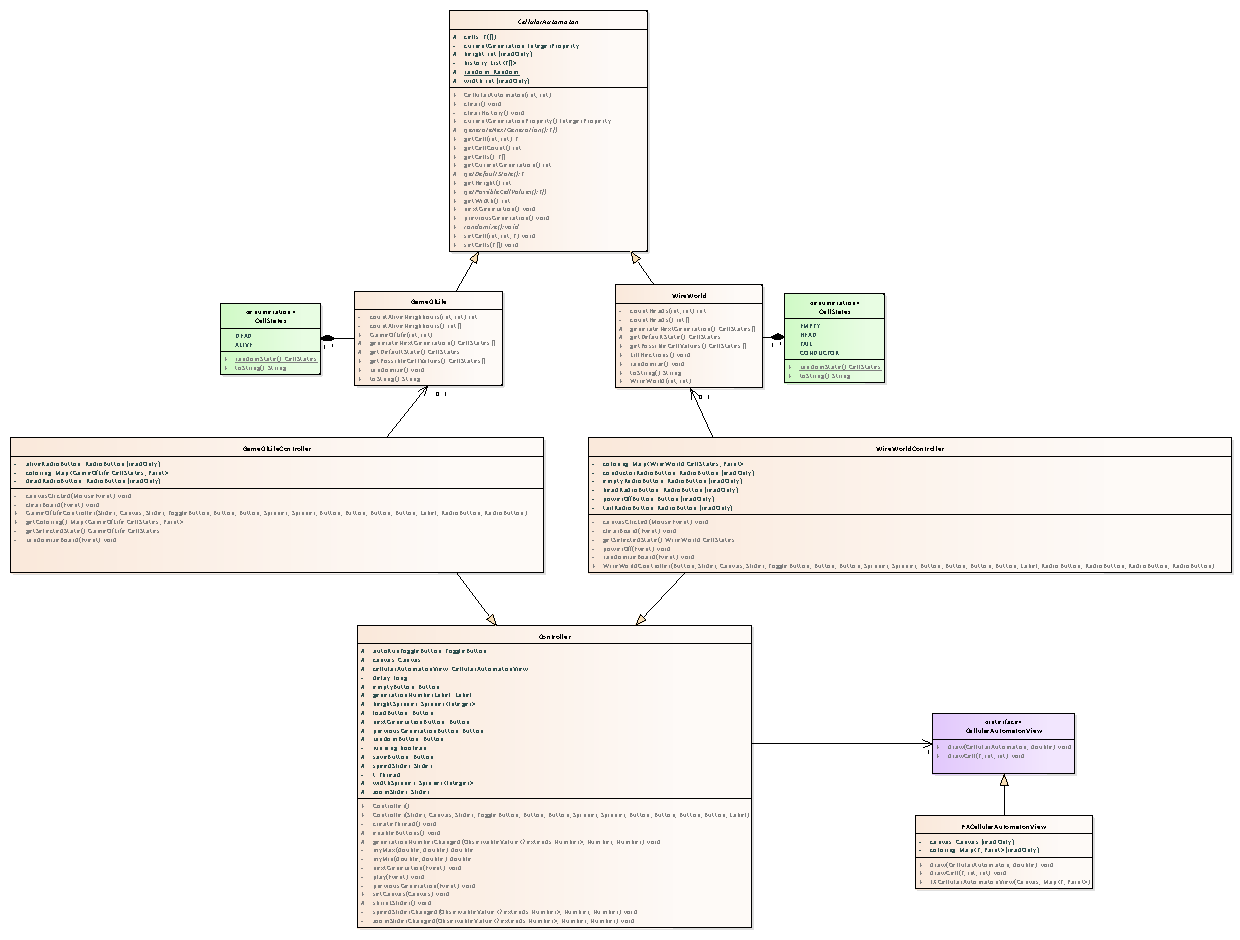
\includegraphics[width=18cm]{Klasy}
	\caption{Diagram klas}	
	%TODO: Wyśrodkować
\end{figure}	

\section{Wzorce projektowe}
%TODO: Opisać zastosowane wzorce

\section{Przepływ sterowania}
%TODO: Opis przepływu sterowania

%TODO: Diagram sekwencji UML

\section{Zastosowane algorytmy}

Obydwa algorytmy muszą przejść przez całą plansze i sprawdzić całe otoczenie (8 komórek) do o koła tej aktualnie rozpatrywanej, co daje nam złożoność 8*n*m, gdzie n to wysokość planszy, m to szerokość planszy, czyli działają w czasie $\Theta$(n*m).

Podczas przeglądania otoczenia komórki, automat przepisuje komórki do tablicy wynikowej lub zmienia ich wartość, zgodnie z zasadami opisanymi w \href{https://github.com/boguszj/Wire-world/blob/master/Specyfikacja-funkcjonalna/Specyfikacja-funkcjonalna.pdf}{Specyfikacji funkcjonalnej}.


\chapter{Opis klas}

\section{Package ,,Controllers''}
Package składający się z klas mających na celu połączenie graficznego interfejsu użytkownika z logiką działania automatów komórkowych. Będzie zawierać 4 klasy, jedną ogólna "CellularAutomatonController", łączącą w sobie cechy wspólne obsługi interfejsu obydwu automatów, oraz z dwóch klas dziedziczących z poprzedniej, zawierających elementu różne dla GameOfLife i WireWorld. Ostatnia z klas będzie pełniła rolę pośrednika między resztą klas a widokiem z pliku \texttt{.fxml}.

\subsection{SetupController}
Klasa będąca punktem startowym programu. Jej zadaniem będzie przekazanie referencji do elementów interfejsu kontrolerom konkretnych zakładek.

\subsection{CellularAutomatonController} %TODO Przerobic 3 pierwsze kontrolery żeby zrobić 1 abstrakcyjny
\texttt{public abstract class CellularAutomatonController<T extends Enum>}
Klasa łącząca w sobie wspólne cechy kontrolerów obydwu automatów skończonych - opisująca powtarzające się elementy graficznego interfejsu użytkownika i ich funkcjonalności.
\subsubsection{Pola}
\paragraph{Pola chronione:}
\begin{itemize}
	\item \texttt{protected Canvas canvas} - płótno na którym rysowana będzie plansza,
	\item \texttt{protected Slider zoomSlider} - suwak reprezentujący przybliżenie planszy \label{sec:zoomSlider},
	\item \texttt{protected Slider speedSlider} - suwak reprezentujący prędkość wyświetlania kolejnych generacji w trybie automatycznym\label{sec:speedSlider},
	\item \texttt{protected ToggleButton autoRunToggleButton} - przycisk włączający i wyłączający tryb automatyczny,
	\item \texttt{protected Button nextGeneration} - przycisk służący do stworzenia i wyświetlenia kolejnej generacji,
	\item \texttt{protected Button previousGeneration}  - przycisk służący do  wyświetlenia poprzedniej generacji,
	\item \texttt{protected Spinner$<$Integer$>$  widthSpinner} - pole reprezentujące szerokość generowanej planszy,
	\item \texttt{protected Spinner$<$Integer$>$ heightSpinner} - pole reprezentujące wysokość generowanej planszy,
	\item \texttt{protected Button RandomButton} - przycisk służący do wygenerowania i wyświetlenia losowej planszy początkowej,
	\item \texttt{protected Button EmptyButton} - przycisk służący do wygenerowania i wyświetlenia pustej planszy początkowej,
	\item \texttt{protected Button saveButton} - przycisk służący do zapisania aktualnego stanu planszy,
	\item \texttt{protected Button loadButton} - przycisk służący do wczytania planszy,
	\item \texttt{protected MenuButton menuButton} - przycisk służący do zapisania części planszy lub narysowania i zapisania wzoru,
	\item \texttt{protected Label generationLabel} -  napis reprezentujący numer aktualnie wyświetlanej generacji,
	\item \texttt{protected CellularAutomatonView cellularAutomatonView} - obiekt odpowiedzialny za narysowanie planszy.
\end{itemize}

\paragraph{Pola prywatne:}
\begin{itemize}
	\item \texttt{private Boolean running} - zmienna typu prawda/fałsz, określająca czy tryb automatyczny jest włączony,
	\item \texttt{private Thread t} - wątek w którym generowane i wyświetlane są kolejne pokolenia w trybie automatycznym\label{sec:thread},
	\item \texttt{private long delay} - odstęp czasowy między wyświetlaniem kolejnych generacji w trybie automatycznym.
\end{itemize}
\subsubsection{Metody}
\paragraph{Konstruktory:}
\begin{itemize}
 	\item \texttt{public Controller(Slider speedSlider, Canvas canvas, Slider zoomSlider, ToggleButton autoRunToggleButton, Button previousGenerationButton, Button nextGenerationButton, Spinner widthSpinner, Spinner heightSpinner, Button randomButton, Button emptyButton, Button saveButton, Button loadButton, Label generationNumberLabel)} - metoda odpowiedzialna za zainicjowanie wszystkich zmiennych, połączenie elementów graficznym z odpowiednimi metodami,
\end{itemize}
\paragraph{Metody publiczne:}
\begin{itemize}
 	\item \texttt{public void setCanvas} - metoda dostępowa pozwalająca ustawić wartość pola \texttt{canvas} funkcjom spoza tego pakietu.
\end{itemize}
\paragraph{Metody chronione:}
\begin{itemize}
 	\item \texttt{protected void shrinkSlider()} - metoda odpowiedzialna za dopasowanie maksymalnej wartość suwaka przybliżenia, tak aby 		wielkość wyświetlanego obrazu mieściła się w maksymalnym rozmiarze płótna,
 	\item \texttt{protected void enableButtons()} - metoda odpowiedzialna za aktywowanie przycisków, które przy starcie programu były 			nieaktywne ze względu na brak funkcjonalności,
 	\item \texttt{protected generationNumberChanged(ObservableValue<? extends Number> observable, Number oldValue, Number newValue)} - metoda odpowiedzialna za aktywowanie i dezaktywowanie przycisku 							\texttt{previousGeneration}, gdy wyświetlenie poprzedniej generacji jest nie możliwe.
\end{itemize}
\paragraph{Metody prywatne:}
\begin{itemize}
 	\item \texttt{private createThread()} - metoda odpowiedzialna za stworzenie nowego wątku \hyperref[sec:thread]{t},
 	\item \texttt{private zoomSliderChanged(ObservableValue<? extends Number> observable, Number oldValue, Number newValue)} - metoda odpowiedzialna za zmianę rozmiaru rysowanych komórek, na podstawie wartości \hyperref[sec:zoomSlider]{suwaka przybliżenia},
 	\item \texttt{private speedSliderChanged(ObservableValue<? extends Number> observable, Number oldValue, Number newValue)} - metoda odpowiedzialna za zmianę prędkości generowania i wyświetlania kolejnych generacji, na podstawie wartości \hyperref[sec:speedSlider]{suwaka prędkości},
 	\item \texttt{private void nextGeneration(Event event)} - metoda odpowiedzialna za przekazanie informacji do modelu automatu komórkowego, o tym że należy wygenerować następne pokolenie,
 	\item \texttt{private void previousGeneration(Event event)} - metoda odpowiedzialna za przekazanie informacji do modelu automatu komórkowego, o tym że należy wygenerować poprzednie pokolenie,
 	\item \texttt{private play()} - metoda odpowiedzialna za uruchomienie tryb automatycznego.
\end{itemize}

\subsection{GameOfLifeController}
Klasa opisująca części kontrolera specyficzne dla automatu GameOfLife.
\subsubsection{Pola}
\paragraph{Pola chronione:}
\begin{itemize}	\label{sec:checkbox}
	\item \texttt{private RadioButton aliveRadioButton} - checkbox oznaczający, że rysowane komórki będą żywe,
	\item \texttt{private RadioButton deadRadioButton} - checkbox oznaczający, że rysowane komórki będą martwe.
\end{itemize}

\paragraph{Pola prywatne:}
\begin{itemize}
	\item \texttt{private Map<GameOfLife.CellStates, Paint> coloring} - mapa przyporządkowująca stanowi automatu kolor (czarny - martwa komórka, biały - żywa komórka).
\end{itemize}
\subsubsection{Funkcje}
\paragraph{Konstruktory:}
\begin{itemize}
\item \texttt{public GameOfLifeController(Slider speedSlider, Canvas canvas, Slider zoomSlider, ToggleButton autoRunToggleButton, Button previousGenerationButton, Button nextGenerationButton, Spinner widthSpinner, Spinner heightSpinner, Button randomButton, Button emptyButton, Button saveButton, Button loadButton, Label generationNumberLabel, RadioButton aliveRadioButton, RadioButton deadRadioButton)} - inicjuje wszystkie zmienne, łączy elementy graficzne z odpowiednimi funkcjami.
\end{itemize}
\paragraph{Metody publiczne:}
\begin{itemize}
 	\item \texttt{public Map<GameOfLife.CellStates, Paint> getColoring()} - metoda dostępowa pozwalająca ustawić wartość pola \texttt{coloring} funkcjom spoza tego pakietu.
\end{itemize}
\paragraph{Metody prywatne:}
\begin{itemize}
 	\item \texttt{ private void randomizeBoard(Event event)} - metoda odpowiedzialna za stworzenie modelu GameOfLife z losowo wygenerowaną planszą początkową,
 	\item \texttt{ private void clearBoard(Event event)} - metoda odpowiedzialna za stworzenie modelu GameOfLife z pustą planszą początkową,
 	\item \texttt{private void canvasClicked(Event event)} metoda odpowiedzialna za przekazanie informacji do modelu automatu komórkowego, o tym że należy na podstawie zaznaczonych \hyperref[sec:checkbox]{checkbox'ów} należy zmienić stan odpowiedniej komórki oraz ją narysować,
 	\item \texttt{private GameOfLife.CellStates getSelectedState()} - metoda odpowiedzialna za pobranie aktualnie wybranego stanu na podstawie zaznaczonych  zaznaczonych \hyperref[sec:checkbox]{checkbox'ów}.
\end{itemize}

\subsection{WireWorldController}
Klasa opisująca części kontrolera specyficzne dla automatu WireWorld.
\subsubsection{Pola}
\paragraph{Pola chronione:}
\begin{itemize}	\label{sec:checkbox}
	\item \texttt{private RadioButton emptyRadioButton} - checkbox oznaczający, że rysowane komórki będą puste,
	\item \texttt{private RadioButton headRadioButton} - checkbox oznaczający, że rysowane komórki będą głowami elektronu,
	\item \texttt{private RadioButton tailRadioButton} - checkbox oznaczający, że rysowane komórki będą ogonami elektronu,
	\item \texttt{private RadioButton conductorRadioButton} - checkbox oznaczający, że rysowane komórki będą przewodnikami,
	\item \texttt{private Button powerOff} - przycisk zamieniający wszystkie komórki będące głowami lub ogonami elektronu na przewodniki.
\end{itemize}

\paragraph{Pola prywatne:}
\begin{itemize}
	\item \texttt{private Map<WireWorld.CellStates, Paint> coloring} - mapa przyporządkowująca stanowi automatu kolor (czerwony - głowa elektronu, niebieski - ogon elektronu, żółty - przewodnik, czarny - pusta komórka).
\end{itemize}
\subsubsection{Funkcje}
\paragraph{Konstruktory:}
\begin{itemize}
\item \texttt{public WireWorld(Button powerOff, Slider speedSlider, Canvas canvas, Slider zoomSlider, ToggleButton autoRunToggleButton, Button previousGenerationButton, Button nextGenerationButton, Spinner widthSpinner, Spinner heightSpinner, Button randomButton, Button emptyButton, Button saveButton, Button loadButton, Label generationNumberLabel, RadioButton emptyRadioButton, RadioButton tailRadioButton, , RadioButton headRadioButton, , RadioButton conductorRadioButton)} - inicjuje wszystkie zmienne, łączy elementy graficzne z odpowiednimi funkcjami.
\end{itemize}
\paragraph{Metody publiczne:}
\begin{itemize}
 	\item \texttt{public Map<WireWorld.CellStates, Paint> getColoring()} - metoda dostępowa pozwalająca ustawić wartość pola \texttt{coloring} funkcjom spoza tego pakietu.
\end{itemize}
\paragraph{Metody prywatne:}
\begin{itemize}
 	\item \texttt{ private void randomizeBoard(Event event)} - metoda odpowiedzialna za stworzenie modelu WireWorld z losowo wygenerowaną planszą początkową,
 	\item \texttt{ private void clearBoard(Event event)} - metoda odpowiedzialna za stworzenie modelu WireWorld z pustą planszą początkową,
 	\item \texttt{private void canvasClicked(Event event)} metoda odpowiedzialna za przekazanie informacji do modelu automatu komórkowego, o tym że należy na podstawie zaznaczonych \hyperref[sec:checkbox]{checkbox'ów} należy zmienić stan odpowiedniej komórki oraz ją narysować,
 	\item \texttt{private GameOfLife.CellStates getSelectedState()} - metoda odpowiedzialna za pobranie aktualnie wybranego stanu na podstawie zaznaczonych  zaznaczonych \hyperref[sec:checkbox]{checkbox'ów},
 	\item \texttt{private void powerOff(Event event)} - metoda odpowiedzialna za przekazanie informacji do modelu automatu komórkowego o tym, że należy zamienić wszystkie komórki będące głowami i ogonami elektronu na przewodniki.
\end{itemize}
\subsection{PatternsController}
\texttt{public abstract class PatternsController<T extends Enum>}
Klasa łącząca w sobie wspólne cechy kontrolerów edytorów wzorów do obydwu automatów komórkowych.
\subsubsection{Pola}
\paragraph{Pola chronione:}
\begin{itemize}
	\item \texttt{protected Canvas canvas} - płótno na którym rysowana będzie plansza,
	\item \texttt{protected Slider zoomSlider} - suwak reprezentujący przybliżenie planszy,
	\item \texttt{protected Spinner$<$Integer$>$  widthSpinner} - pole reprezentujące szerokość generowanej planszy,
	\item \texttt{protected Spinner$<$Integer$>$ heightSpinner} - pole reprezentujące wysokość generowanej planszy,
	\item \texttt{protected Button EmptyButton} - przycisk służący do wygenerowania i wyświetlenia pustej planszy początkowej,
	\item \texttt{protected Button saveButton} - przycisk służący do zapisania wzoru,
	\item \texttt{protected Button loadButton} - przycisk służący do wczytania wzoru,
	\item \texttt{protected T[] cellStates} - tablica reprezentująca tablicę stanów automatu,
	\item \texttt{protected CellularAutomatonView cellularAutomatonView} - obiekt odpowiedzialny za narysowanie planszy.
\end{itemize}

\paragraph{Pola prywatne:}
\begin{itemize}
	\item \texttt{private Map<T, Paint> colouring} - mapa przyporządkowująca stanowi automatu kolor.
\end{itemize}
\subsubsection{Funkcje}
\paragraph{Konstruktory:}
\begin{itemize}
\item \texttt{public WireWorld(Button powerOff, Slider speedSlider, Canvas canvas, Slider zoomSlider, Spinner widthSpinner, Spinner heightSpinnr, Button emptyButton, Button saveButton, Button loadButton, T[] CellStates, CellularAutomatonView cellularAutomatonView)} - inicjuje wszystkie zmienne, łączy elementy graficzne z odpowiednimi funkcjami.
\end{itemize}
\paragraph{Metody prywatne:}
\begin{itemize}
 	\item \texttt{ private abstract void clearBoard(Event event)} - metoda odpowiedzialna za stworzenie i narysowanie pustej planszy odpowiedniego automatu komórkowego.
 	\item \texttt{private void canvasClicked(Event event)} metoda odpowiedzialna za zmianę stanu komórki na podstawie zaznaczonych checkbox'ów i przekazanie informacji o tym że, trzeba ją narysować.
 	\item \texttt{private abstract T getSelectedState()} - metoda odpowiedzialna za pobranie aktualnie wybranego stanu na podstawie zaznaczonych  zaznaczonych \hyperref[sec:checkbox]{checkbox'ów},
 	\item \texttt{private void save()} - metoda odpowiedzialna za zapis wzoru.
\end{itemize}

\subsection{GameOfLifePatternsController}
\texttt{public class GameOfLifePatternsController extends PatternsController<GameOfLife.CellStates>}
Klasa opisująca części kontrolera specyficzne dla edytora wzorów automatu komórkowego GameOfLife.
\subsubsection{Pola}
\paragraph{Pola prywatne:}
\begin{itemize}	\label{sec:checkbox}
	\item \texttt{private RadioButton deadRadioButton} - checkbox oznaczający, że rysowane komórki będą martwe,
	\item \texttt{private RadioButton aliveRadioButton} - checkbox oznaczający, że rysowane komórki będą żywe.
\end{itemize}

\subsubsection{Metody}
\paragraph{Konstruktory:}
\begin{itemize}
\item \texttt{public WireWorldPatternsController(Button powerOff, Slider speedSlider, Canvas canvas, Slider zoomSlider, Spinner widthSpinner, Spinner heightSpinner, Button emptyButton, Button saveButton, Button loadButton, RadioButton aliveRadioButton, RadioButton deadRadioButton, T[] CellStates, CellularAutomatonView cellularAutomatonView)} - inicjuje wszystkie zmienne, łączy elementy graficzne z odpowiednimi funkcjami.
\end{itemize}
\paragraph{Klasa implementuje poniższe metody abstrakcyjne z klasy bazowe:}
\begin{itemize}
 	\item \texttt{private void clearBoard(Event event)},
 	\item \texttt{private T getSelectedState()}.
\end{itemize}
Szczegółowy opis każdej z metod znajduje się w klasie bazowej \hyperref[subsec:cellularAutomaton]{WireWorldPatternsController}.

\subsection{WireWorldPatternsController}
\texttt{public class WireWorldPatternsController extends PatternsController<WireWorld.CellStates>}
Klasa opisująca części kontrolera specyficzne dla edytora wzorów automatu komórkowego WireWorld.
\subsubsection{Pola}
\paragraph{Pola prywatne:}
\begin{itemize}	\label{sec:checkbox}
	\item \texttt{private RadioButton emptyRadioButton} - checkbox oznaczający, że rysowane komórki będą puste,
	\item \texttt{private RadioButton headRadioButton} - checkbox oznaczający, że rysowane komórki będą głowami elektronu,
	\item \texttt{private RadioButton tailRadioButton} - checkbox oznaczający, że rysowane komórki będą ogonami elektronu,
	\item \texttt{private RadioButton conductorRadioButton} - checkbox oznaczający, że rysowane komórki będą przewodnikami,
\end{itemize}

\subsubsection{Metody}
\paragraph{Konstruktory:}
\begin{itemize}
\item \texttt{public WireWorldPatternsController(Button powerOff, Slider speedSlider, Canvas canvas, Slider zoomSlider, Spinner widthSpinner, Spinner heightSpinner, Button emptyButton, Button saveButton, Button loadButton, RadioButton emptyRadioButton, RadioButton tailRadioButton, , RadioButton headRadioButton, , RadioButton conductorRadioButton, T[] CellStates, CellularAutomatonView cellularAutomatonView)} - inicjuje wszystkie zmienne, łączy elementy graficzne z odpowiednimi funkcjami.
\end{itemize}
\paragraph{Klasa implementuje poniższe metody abstrakcyjne z klasy bazowe:}
\begin{itemize}
 	\item \texttt{private void clearBoard(Event event)},
 	\item \texttt{private T getSelectedState()}.
\end{itemize}
Szczegółowy opis każdej z metod znajduje się w klasie bazowej \hyperref[subsec:cellularAutomaton]{WireWorldPatternsController}.
\section{Pakiet ,,Models''}
Pakiet składający się z klas reprezentujących odpowiednie automaty komórkowe, odpowiedzialnych za przechowywanie ich zasad, przeprowadzanie symulacji i generowanie kolejnych pokoleń. Będzie on zawierać 3 klasy, jedną ogólną \texttt{CellularAutomaton}, łączącą w sobie cechy wspólne wszystkich automatów komórkowych oraz 2 klasy dziedziczące z poprzedniej, opisujące działanie konkretnych automatów (\texttt{GameOfLife} oraz \texttt{WireWorld}).

\subsection{CellularAutomaton} \label{subsec:cellularAutomaton}
\texttt{public abstract class CellularAutomaton<T extends Enum>}

Klasa abstrakcyjna reprezentująca dowolny automat komórkowy.
Typ \texttt{T} jest typem wyliczeniowym możliwych stanów komórki automatu.

\paragraph{Konstruktory:}
\begin{itemize}
	\item \texttt{public CellularAutomaton(int width, int height)} -- Tworzy automat o podanym rozmiarze z komórkami o domyślnym stanie.
\end{itemize}

\paragraph{Pola chronione:}
\begin{itemize}
	\item \texttt{protected final int width} -- Liczba kolumn planszy automatu,
	\item \texttt{protected final int height} -- Liczba wierszy planszy automatu,
	\item \texttt{protected T[] cells} -- Tablica wszystkich komórek automatu,
	\item \texttt{protected static Random random} -- Zmienna używana do losowania stanów.
\end{itemize}

\paragraph{Pola prywatne:}
\begin{itemize}
	\item \texttt{private List<T[]> history} -- Lista poprzednich stanów automatu. \\ Umożliwia przejście od poprzedniego stanu,
	\item \texttt{private IntegerProperty currentGeneration} -- Liczba reprezentująca number aktualnego pokolenia automatu.
\end{itemize}

\paragraph{Metody publiczne:}
\begin{itemize}
	\item \texttt{public abstract T[] getPossibleCellValues()} -- Zwraca tablicę możliwych stanów komórki automatu,
	\item \texttt{public void setCells(T[] cells)} -- Ustawia wszystkie komórki automatu na nowe wartości,
	\item \texttt{public T getCell(int row, int column)} -- Zwraca wartość konkretnej komórki,
	\item \texttt{public int getCellCount()} -- Zwraca ilość komórek w automacie,
	\item \texttt{public void nextGeneration()} -- Przeprowadza automat do następnego stanu,
	\item \texttt{public void previousGeneration()} -- Przeprowadza automat do poprzedniego stanu
	\item \texttt{public void clear()} -- Ustawia stan wszystkich komórek na domyślny,
	\item \texttt{public abstract void randomize()} -- Ustawia stan wszystkich komórek na losowy.
\end{itemize}

\paragraph{Metody chronione:}
\begin{itemize}
	\item \texttt{protected abstract T[] generateNextGeneration()} -- Zwraca stany komórek następnej generacji,
	\item \texttt{protected abstract T getDefaultState()} -- Zwraca domyślny stan dla danego automatu.
\end{itemize}

\paragraph{Metody prywatne:}
\begin{itemize}
	\item \texttt{private void clearHistory()} -- Ustawia aktualny stan automatu jako jedyny stan w historii.
\end{itemize}

\subsection{GameOfLife}
\texttt{public class GameOfLife extends CellularAutomaton<GameOfLife.CellStates>}

Klasa jest konkretną implementacja automatu komórkowego \textit{Game of Life}.

\paragraph{Klasy wewnętrzne:} \mbox{} \\
Typ wyliczeniowy reprezentujący możliwe stany komórki.
\begin{verbatim}
public enum CellStates {
    DEAD,
    ALIVE;

    public static CellStates randomState() - Zwraca losowy stan komórki.
}
\end{verbatim}

\paragraph{Konstruktory:}
\begin{itemize}
	\item \texttt{public GameOfLife(int width, int height)} -- Tworzy automat o podanym rozmiarze z komórkami o domyślnym stanie.
\end{itemize}

\paragraph{Metody prywatne:}
\begin{itemize}
    \item \texttt{private int[] countAliveNeighbours()} -- Oblicza ilość żywych sąsiadów dla każdej komórki automatu,
    \item private int countAliveNeighbours(final int cellX, final int cellY) -- Oblicza ilość żywych sąsiadów dla konkretnej komórki automatu.
\end{itemize}

\paragraph{Klasa implementuje poniższe metody abstrakcyjne z klasy bazowe:}
\begin{itemize}
    \item \texttt{CellStates[] getPossibleCellValues()},
    \item \texttt{protected CellStates[] generateNextGeneration()},
    \item \texttt{public void randomize()},
    \item \texttt{protected CellStates getDefaultState()}.
\end{itemize}
Szczegółowy opis każdej z metod znajduje się w klasie bazowej \hyperref[subsec:cellularAutomaton]{CellularAutomaton}.

\subsection{WireWorld}
\texttt{public class WireWorld extends CellularAutomaton<WireWorld.CellStates>}

Klasa jest konkretną implementacja automatu komórkowego \textit{WireWorld}.

\paragraph{Klasy wewnętrzne:} \mbox{} \\
Typ wyliczeniowy reprezentujący możliwe stany komórki.
\begin{verbatim}
public enum CellStates {
    EMPTY,
    HEAD,
    TAIL,
    CONDUCTOR;

    public static CellStates randomState() - Zwraca losowy stan komórki.
}
\end{verbatim}

\paragraph{Konstruktory:}
\begin{itemize}
	\item \texttt{public WireWorld(int width, int height)} -- Tworzy automat o podanym rozmiarze z komórkami o domyślnym stanie.
\end{itemize}

\paragraph{Metody publiczne:}
\begin{itemize}
    \item \texttt{public void killElectrons()} -- Zamienia wszystkie głowy elektronów i ogony elektronów na przewodniki.
\end{itemize}

\paragraph{Metody prywatne:}
\begin{itemize}
    \item \texttt{private int countHeads(final int cellX, final int cellY)} -- Oblicza ilość sąsiadów konkretnej komórki będących głową elektronu,
    \item \texttt{private int[] countHeads()} -- Dla każdej komórki oblicza ilość sąsiadów będących głową elektronu.
\end{itemize}

\paragraph{Klasa implementuje poniższe metody abstrakcyjne z klasy bazowe:}
\begin{itemize}
    \item \texttt{CellStates[] getPossibleCellValues()},
    \item \texttt{protected CellStates[] generateNextGeneration()},
    \item \texttt{public void randomize()},
    \item \texttt{protected CellStates getDefaultState()}.
\end{itemize}
Szczegółowy opis każdej z metod znajduje się w klasie bazowej \hyperref[subsec:cellularAutomaton]{CellularAutomaton}.

\section{Pakiet ,,Views''}
Pakiet składający się z interfejsu generalizującego wyświetlanie planszy, który umożliwia dołączanie do projektu nowych implementacji wizualizacji automatu komórkowego oraz z klasy implementującej ten interfejs, renderującej widok 2D przy użyciu obiektu Canvas z biblioteki JavaFX.
\subsection{CellularAutomatonView}
Interfejs generalizujący wizualizacje planszy.
\paragraph{Metody publiczne:}
\begin{itemize}
	\item \texttt{public void drawCell(T CellState, final int x, final int y, final double cellSize)} - metoda rysująca pojedynczą komórkę,
	\item \texttt{public void draw(CellularAutomaton ca, final double cellSize)} - metoda rysująca całą planszę, na podstawie tablicy komórek.
\end{itemize}
\subsection{FXCellularAutomatonView}
Implementacja interfejsu \texttt{CellularAutomatonView} przy użyciu obiektu Canvas z biblioteki JavaFX. Wizualizacja 2D automatu komórkowego.
\subsubsection{Pola}
\paragraph{Pola prywatne:}
\begin{itemize}
	\item \texttt{private final Canvas canvas} - płótno, na którym rysowana będzie plansza z aktualnym stanem automatu komórkowego,
	\item \texttt{private final Map<T, Paint> colouring} - mapa przyporządkowująca stanowi automatu kolor.
\end{itemize}
\paragraph{Konstruktory:}
\begin{itemize}
	\item \texttt{public FXCellularAutomatonView(Canvas canvas, Map<T, Paint> colouring )} - inicjacja pól.
\end{itemize}
\paragraph{Metody publiczne:}
\begin{itemize}
	\item \texttt{public void drawCell(T CellState, final int x, final int y, final double cellSize)} - metoda rysująca pojedynczą komórkę,
	\item \texttt{public void draw(CellularAutomaton ca, final double cellSize)} - metoda rysująca całą planszę, na podstawie tablicy komórek.
\end{itemize}



\chapter{Testy}
%TODO: Opis testów

\chapter{Biblioteki}
%TODO: Opis bibliotek

\end{document}
